
%%%%%%%%%%%%%%%%%%%%%%%%%%%%%%%%%%%%%%%%%%%%%%%%%%%%%%%%%%%%%%%%%%%%%%%%%%%%%%%%%%%%%%%
%%%%%%%%%%%%%%%%%%%%%%%%%%%%%%%%%%%%%%%%%%%%%%%%%%%%%%%%%%%%%%%%%%%%%%%%%%%%%%%%%%%%%%%
% 
% This top part of the document is called the 'preamble'.  Modify it with caution!
%
% The real document starts below where it says 'The main document starts here'.

\documentclass[12pt]{article}

\usepackage{amssymb,amsmath,amsthm}
\usepackage[top=1in, bottom=1in, left=1.25in, right=1.25in]{geometry}
\usepackage{fancyhdr}
\usepackage{enumerate}
\usepackage{listings}
\usepackage{graphicx}
\usepackage{float}
% Comment the following line to use TeX's default font of Computer Modern.
\usepackage{times,txfonts}



\makeatletter
\renewcommand*\env@matrix[1][*\c@MaxMatrixCols c]{%
  \hskip -\arraycolsep
  \let\@ifnextchar\new@ifnextchar
  \array{#1}}
\makeatother

\newtheoremstyle{homework}% name of the style to be used
  {18pt}% measure of space to leave above the theorem. E.g.: 3pt
  {12pt}% measure of space to leave below the theorem. E.g.: 3pt
  {}% name of font to use in the body of the theorem
  {}% measure of space to indent
  {\bfseries}% name of head font
  {:}% punctuation between head and body
  {2ex}% space after theorem head; " " = normal interword space
  {}% Manually specify head
\theoremstyle{homework} 

% Set up an Exercise environment and a Solution label.
\newtheorem*{exercisecore}{Exercise \@currentlabel}
\newenvironment{exercise}[1]
{\def\@currentlabel{#1}\exercisecore}
{\endexercisecore}

\newcommand{\localhead}[1]{\par\smallskip\noindent\textbf{#1}\nobreak\\}%
\newcommand\solution{\localhead{Solution:}}

%%%%%%%%%%%%%%%%%%%%%%%%%%%%%%%%%%%%%%%%%%%%%%%%%%%%%%%%%%%%%%%%%%%%%%%%
%
% Stuff for getting the name/document date/title across the header
\makeatletter
\RequirePackage{fancyhdr}
\pagestyle{fancy}
\fancyfoot[C]{\ifnum \value{page} > 1\relax\thepage\fi}
\fancyhead[L]{\ifx\@doclabel\@empty\else\@doclabel\fi}
\fancyhead[C]{\ifx\@docdate\@empty\else\@docdate\fi}
\fancyhead[R]{\ifx\@docauthor\@empty\else\@docauthor\fi}
\headheight 15pt

\def\doclabel#1{\gdef\@doclabel{#1}}
\doclabel{Use {\tt\textbackslash doclabel\{MY LABEL\}}.}
\def\docdate#1{\gdef\@docdate{#1}}
\docdate{Use {\tt\textbackslash docdate\{MY DATE\}}.}
\def\docauthor#1{\gdef\@docauthor{#1}}
\docauthor{Use {\tt\textbackslash docauthor\{MY NAME\}}.}
\makeatother

% Shortcuts for blackboard bold number sets (reals, integers, etc.)
\newcommand{\Reals}{\ensuremath{\mathbb R}}
\newcommand{\Nats}{\ensuremath{\mathbb N}}
\newcommand{\Ints}{\ensuremath{\mathbb Z}}
\newcommand{\Rats}{\ensuremath{\mathbb Q}}
\newcommand{\Cplx}{\ensuremath{\mathbb C}}
%% Some equivalents that some people may prefer.
\let\RR\Reals
\let\NN\Nats
\let\II\Ints
\let\CC\Cplx

%%%%%%%%%%%%%%%%%%%%%%%%%%%%%%%%%%%%%%%%%%%%%%%%%%%%%%%%%%%%%%%%%%%%%%%%%%%%%%%%%%%%%%%
%%%%%%%%%%%%%%%%%%%%%%%%%%%%%%%%%%%%%%%%%%%%%%%%%%%%%%%%%%%%%%%%%%%%%%%%%%%%%%%%%%%%%%%
% 
% The main document start here.

% The following commands set up the material that appears in the header.
\doclabel{Math 614: Homework 3}
\docauthor{Stefano Fochesatto}
\docdate{\today}

\begin{document}


\begin{exercise}{P8} On page 12 of the textbook, equation (2.4) says $(AB)^* = B^*A^*$.
  Prove this by showing the matrix entries are equal.\\
  \solution Suppose that $A$ is an $mxn$ matrix and $B$ is a $nxl$ matrix. Considering the following $(AB)^*$ using the entry definition of matrix-matrix multiplication
  defined in equation (1.5) we know the following, 
  \begin{equation*}
    ab_{i,j} = \sum_{k = 1}^n a_{i,k}b_{k,j}.
  \end{equation*}
  Taking the adjoint of $AB$ to get $AB^*$ just requires us to swap the indices $i,j$ in the left hand side, 
  \begin{equation*}
    (ab)^*_{j,i} = \sum_{k = 1}^n a_{i,k}b_{k,j}.
  \end{equation*}
  Now we can consider $B^*A^*$ and apply the same formula,
  \begin{equation*}
    (b)^*(a)^*_{i,j} = \sum_{k = 1}^n (b)^*_{i,k}(a)^*_{k,j}.
  \end{equation*}
  Note that the adjoint operation can be described with the following, 
  \begin{equation*}
    b_{i,j} = (b)^*_{j,i},
  \end{equation*}
  \begin{equation*}
    a_{i,j} = (a)^*_{j,i}.
  \end{equation*}
  Thus by substitution the following is true,
  \begin{equation*}
    \sum_{k = 1}^n a_{i,k}b_{k,j} = \sum_{k = 1}^n (b)^*_{k,j}(a)^*_{i,k}.
  \end{equation*}
  Therefore  $(AB)^* = B^*A^*$. 
\end{exercise}
\vspace{.25in}






\begin{exercise}{P9} On page 21 of the textbook, equation (3.10) gives a formula of 
  the $\infty$-norm of an $mxn$ matrix. Let $a_i$ denote the $i^{th}$ row of $A$ and prove it,
  \begin{equation*}
    ||A||_{\infty} = \max_{1 \leq i \leq m}||a_i||_1
  \end{equation*}
  \solution Suppose an $mxn$ matrix $A$. Now consider the
  set $\{x \in \CC^{n}: \max_{1 \leq j \leq n} |x_j|\}$ and note that the set of vectors $Ax$ satisfy,
  \begin{equation*}    
      ||Ax||_{\infty} = ||a^*_ix||_{\infty} \leq \max_{1 \leq i \leq n}||a^*_ix||_{\infty}.
  \end{equation*}
  Choosing $x$ such that all the entries have the property that $|x_i| = 1$ we can maximize each inner product $||a_i||x||$.
  Note that this turns the inner product into the same operation as the one-norm for each $a_i$. Therefore the product 
  $||A||_{\infty}$ attains the upper bound and we get the following,
  \begin{equation*}
  ||A||_{\infty} = \max_{1 \leq i \leq m}||a_i||_1.
  \end{equation*}
\end{exercise}
\vspace{.25in}


\begin{exercise}{2.6} If $u$ and $v$ are $m$-vectors, the matrix $A = I + uv^*$ is known as the 
  rank-one perturbation of the identity. Show that if $A$ is nonsingular, then it's inverse has the form 
  $A^{-1} = I + \alpha uv^*$ for some scalar $\alpha$, and give an expression for $\alpha$. For what 
  $u$ and $v$ is $A$ singular? If it is singular, what is the $null(A)$.\\

  \solution Suppose that $A$ is nonsingular and $u$ and $v$ are $m$-vectors such that $A = I + uv^*$. 
  Consider the following equation for some scalar $\alpha$, 
  \begin{equation*}
    (I + uv^*)(I + \alpha uv^*) = I.
  \end{equation*}
  Expanding the product, 
  \begin{align*}
    (I + uv^*)(I + \alpha uv^*) &= I,\\
    \alpha uv^* + uv^* + uv^*\alpha uv^* + I &= I,\\
    \alpha uv^* + uv^* + \alpha uv^*uv^* &= 0.
  \end{align*}
  Note that $v^*u$ is a scalar, so the following applies,
  \begin{align*}
    \alpha uv^* + uv^* + \alpha u(v^*u)v^* &= 0,\\
    \alpha uv^* + uv^* + \alpha (v^*u)uv^* &= 0,\\
    (\alpha + 1 + \alpha (v^*u))uv^* &= 0.
  \end{align*}
  When $uv^* = 0$ we get the trivial case where $A = I$. Solving the other factor for $\alpha$,
  \begin{align*}
    \alpha + 1 + \alpha (v^*u) &= 0,\\
    \alpha + \alpha (v^*u) &= -1,\\
    \alpha (1+ (v^*u)) &= -1,\\
    \alpha &= \dfrac{-1}{(1+ (v^*u))}.
  \end{align*}
  Thus $A$ has an inverse of the form $I + \alpha uv^*$ when $\alpha = \frac{-1}{(1+ (v^*u))}$ and $v^*u \neq -1$.\\

  To show when $A$ is singular, consider all $u$ and $v$ such that $u^*v = -1$. Implicit in this
  consideration is the fact that $u \neq 0$ and $v \neq 0$. Evaluating $Au$ we get the following, 
  \begin{equation*}
    Au = (I + uv^*)u =  Iu + uv^*u = u + (-1)u = 0.
  \end{equation*}
  Since $u \neq 0$, $A$ must be singular. Furthermore substituting any vector in the $span(u)$
  we also get 0 so by definition $span(u) = Null(A)$.
\end{exercise}
\vspace{.25in}

\begin{exercise}{3.2} Let $||\cdot||$ denote any norm on $\CC^m$ and also the induced matrix norm on $\CC^{mxm}$. 
  Show that $\rho(A) \leq ||A||$, where $\rho(A)$ is the spectral radius of $A$, i.e., the largest absolute value 
  $|\lambda|$ of an eigenvalue $\lambda$ of $A$.\\

  \solution By definition $||A||_{mxm}$ is the supremum of the ratios, $||Ax||_{m}/||x||_{m}$. Now note that by the definition of the eigenvalue,
  for some eigenvector $v$ and the corresponding eigenvalue $\lambda$ we know the following. 
  \begin{equation*}
    Av = \lambda v.
  \end{equation*}
  Taking the norm of both sides we get, 
  \begin{equation*}
    ||Av||_{m}=||\lambda v||_{m}.
  \end{equation*}
  Applying the linearity of vector norms, and solving for $|\lambda|$,
  \begin{align*}
    ||Av||_{m}&=|\lambda |||v||_{m},\\
    \dfrac{||Av||_{m}}{||v||_{m}}&=|\lambda|.
  \end{align*}
  Consider some $\hat{v}$ such that $|\lambda|$ is maximized and we get that, 
  \begin{equation*}
    \rho(A) = \max |\lambda| = \dfrac{||A\hat{v}||_{m}}{||\hat{v}||_{m}}.
  \end{equation*}
  Thus by definition $\rho(A)$ is contained in the set of all ratios $||Ax||_{m}/||x||_{m}$, where 
  $||A||_{mxm}$ is the supremum, therefore we know
  \begin{equation*}
  \rho(A) \leq ||A||.
  \end{equation*}
\end{exercise}
\vspace{.25in}



\begin{exercise}{3.3} Vector and matrix $p$-norms are related by various inequalities, often involving
  the dimensions $m$ or $n$. For each of the following, verify the inequality and give an example of a 
  nonzero vector or matrix (for general $m$,$n$) for which the equality is achieved. 
  In this problem $x$ is an $m$-vector and $A$ is an $mxn$ matrix.\\
  \begin{enumerate}
    \item $||x||_{\infty} \leq ||x||_2$\\
    \solution Consider the definition of the vector $\infty$-norm, 
    \begin{equation*}
      ||x||_{\infty} = \max_{1 \leq i \leq m} |x_i|.
    \end{equation*}
    Clearly we can replace the absolute value operator by squaring then square-rooting the max term. 
    Doing so we get the following, 
      \begin{equation*}
        ||x||_{\infty} = \max_{1 \leq i \leq m} \sqrt{(x_i)^2}.
      \end{equation*}
      If we add the square of the remaining $x_i$ terms it must be the case that we produce a sum larger 
      than just the maximum $x_i$ term, thus
      \begin{equation*}
        ||x||_{\infty} = \max_{1 \leq i \leq m} \sqrt{(x_i)^2} \leq \sqrt{\sum_{i=1}^m (x_i)^2} = ||x||_2.
      \end{equation*}
      For an example consider the vector $\hat{x} = [2, 1]$ and note that $||\hat{x}||_{\infty} = 2 \leq \sqrt{5} = ||\hat{x}||_{2}$
    \vspace{.15in}



    \item $||x||_{2} \leq \sqrt{m}||x||_{\infty}$\\
    \solution Consider the definition of the vector $2$-norm. 
    \begin{equation*}
      ||x||_2 = \sqrt{\sum_{i=1}^m (x_i)^2}.
    \end{equation*}
    Replacing every $x_i$ in the sum with the $\max_{1 \leq i \leq m} x_i$ we get the following, 
    \begin{equation*}
      ||x||_{2} \leq \sqrt{\sum_{i=1}^m (\max_{1 \leq i \leq m} x_i)^2} = \sqrt{m(\max_{1 \leq i \leq m} x_i)^2} = \sqrt{m} \max_{1 \leq i \leq m}|x_i| = \sqrt{m}||x||_{\infty}.
    \end{equation*}
    For an example we can once again consider $\hat{x} = [2, 1]$ and note that $||\hat{x}||_{2} = \sqrt{5} \leq \sqrt{2}*2 = \sqrt{m}||\hat{x}||_{\infty}$.
    \vspace{.15in}
  \end{enumerate}
  
\end{exercise}
\vspace{.25in}



\begin{exercise}{4.3} Write a MATLAB program which, given a real $2x2$ matrix $A$, plots the right singular 
  vectors $v_1$, and $v_2$ in the unit circle and also the left singular vectors $u_1$ and $u_2$ in the appropriate ellipse, 
  as in Figure $4.1$. Apply your program to the matrix $(3.7)$ and also to the $2x2$ matrices in Exercise $4.1$
  \solution 
  \textbf{Code:}
          \begin{center}
            \lstinputlisting{vismat.m}
          \end{center}

          \begin{figure}[H]
            \begin{center}
              \caption{Vismat() with matrix from 3.7 [1 2;0 2]}
              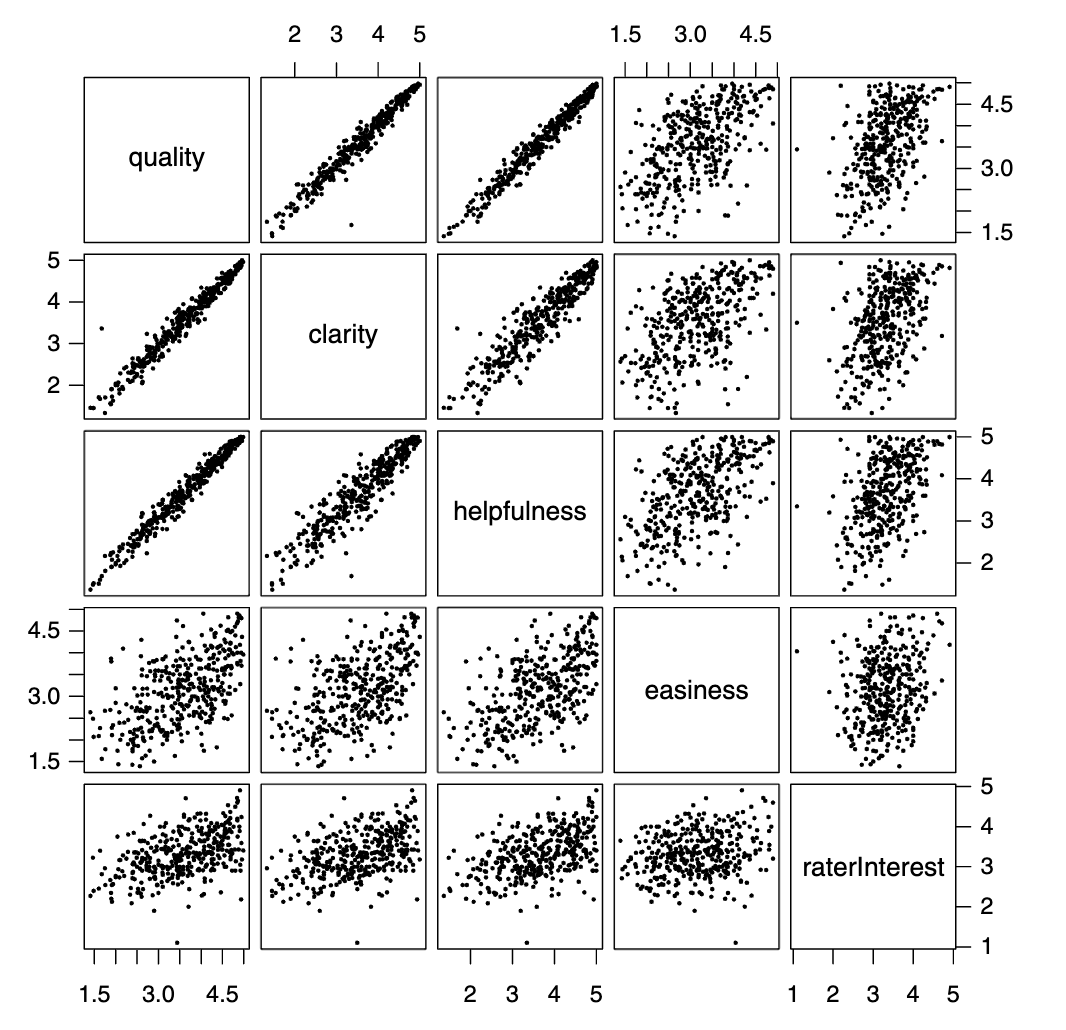
\includegraphics[width=.75\textwidth]{plot1.png}
            \end{center}
          \end{figure}

          \begin{figure}[H]
            \begin{center}
              \caption{Vismat(A) with matrix from 4.1 [3 0;0 -2]}
              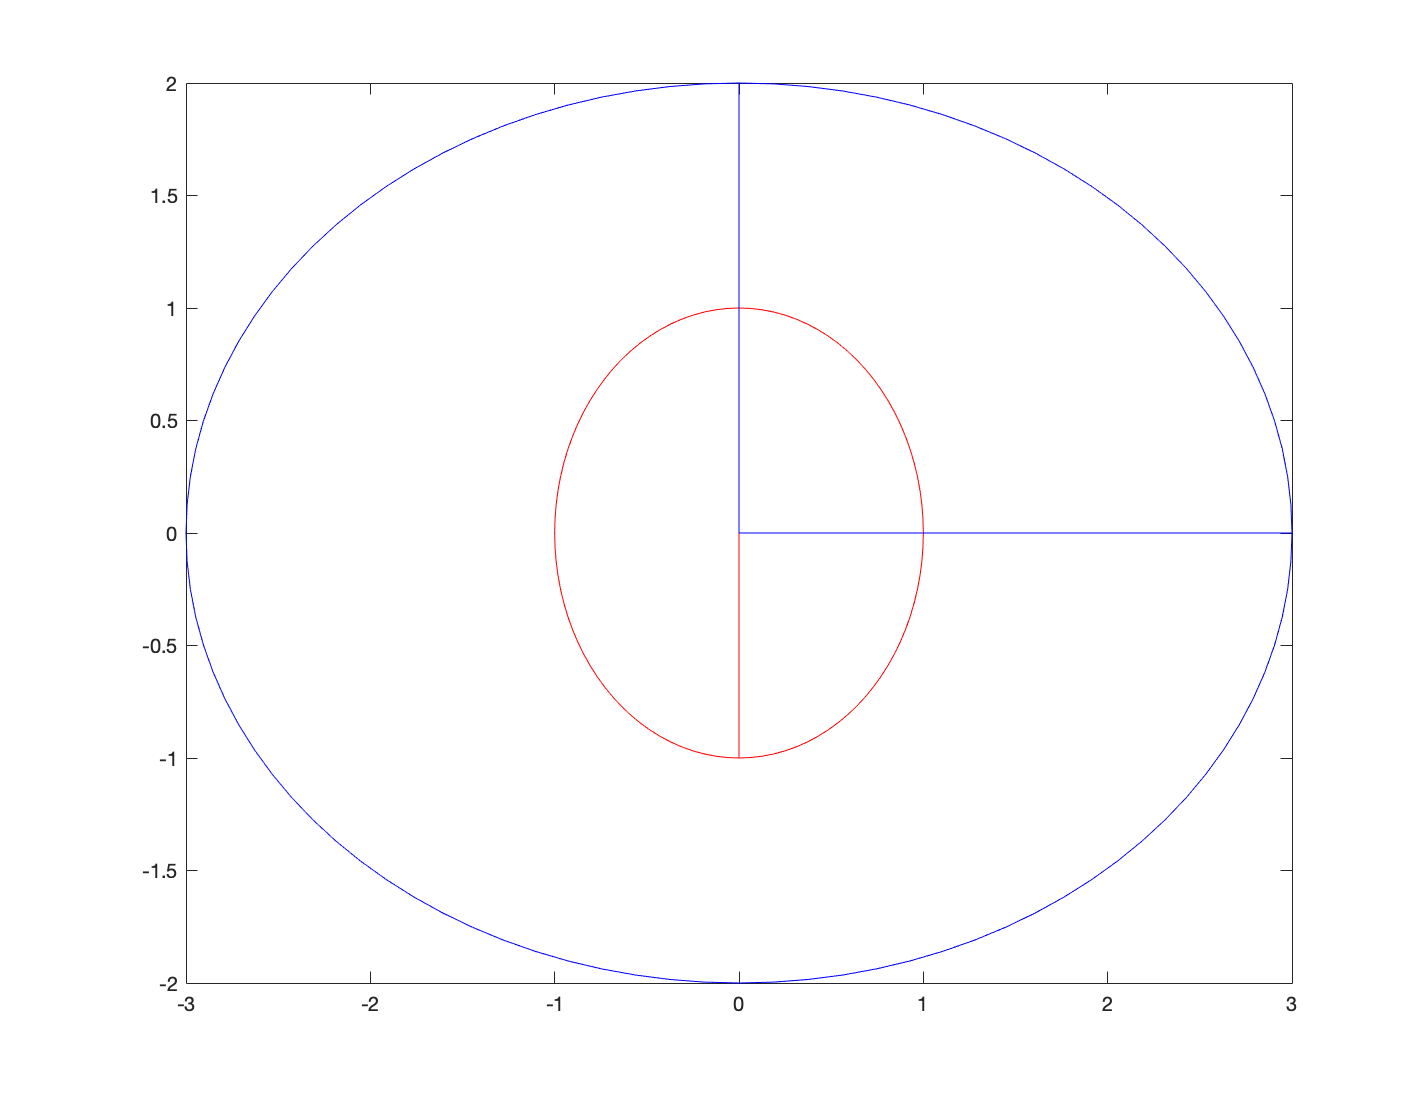
\includegraphics[width=.75\textwidth]{plot2.png}
            \end{center}
          \end{figure}
          \begin{figure}[H]
            \begin{center}
              \caption{Vismat(A) with matrix from 4.1 [2 0;0 3]}
              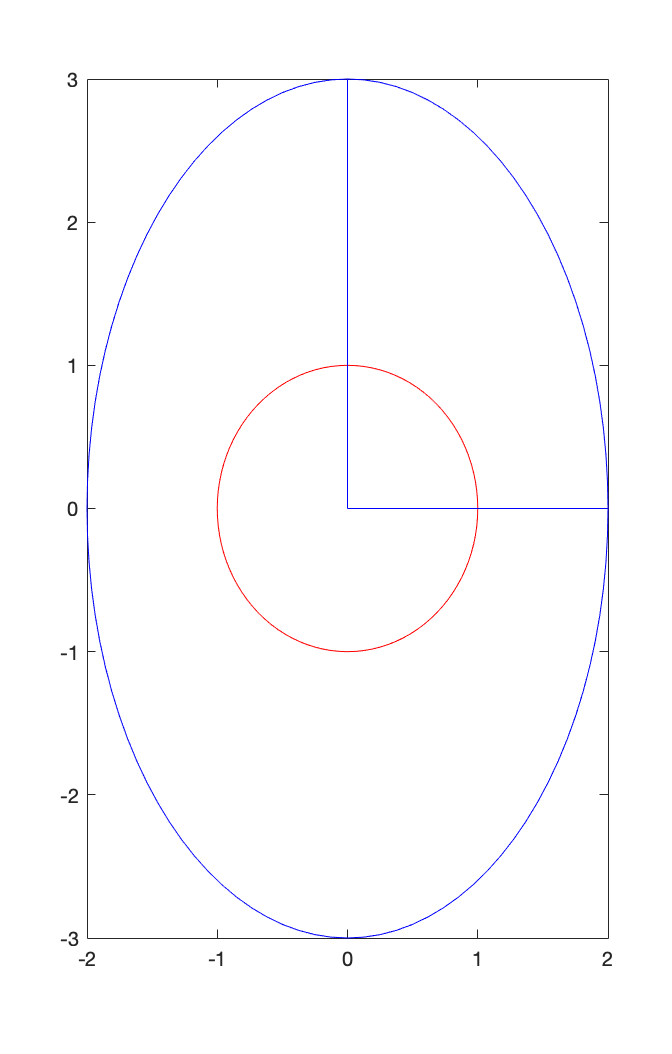
\includegraphics[width=.75\textwidth]{plot3.png}
            \end{center}
          \end{figure}
          \begin{figure}[H]
            \begin{center}
              \caption{Vismat(A) with matrix from 4.1 [1 1;0 0]}
              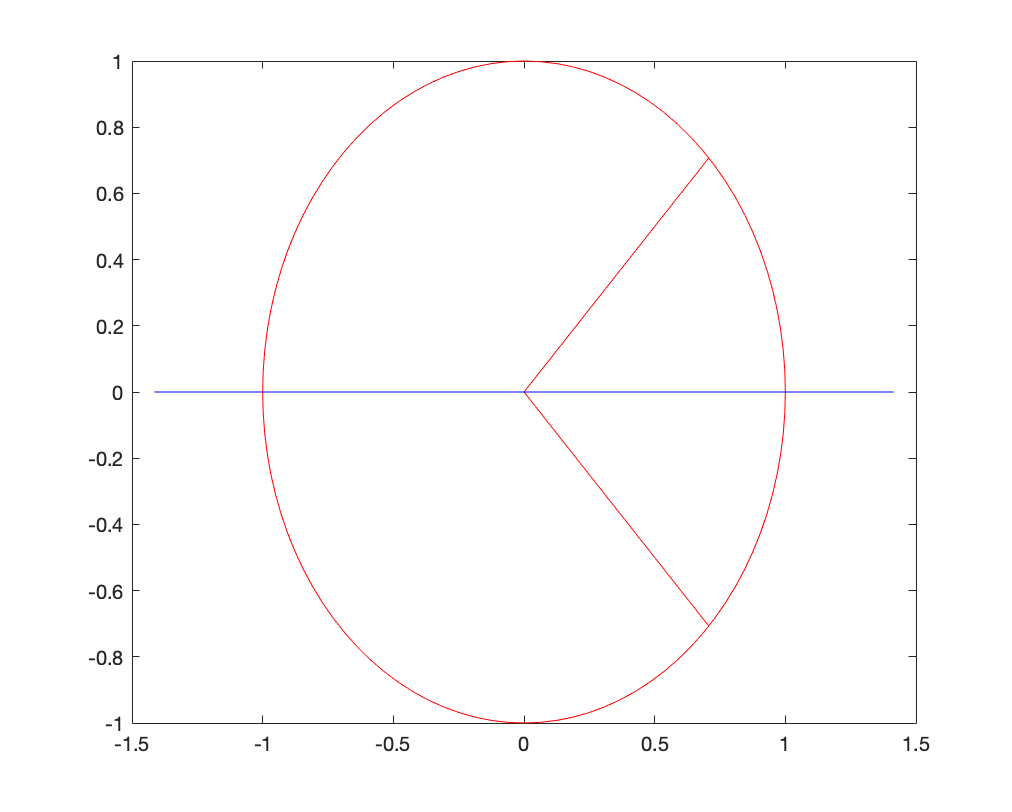
\includegraphics[width=.75\textwidth]{plot4.png}
            \end{center}
          \end{figure}
          \begin{figure}[H]
            \begin{center}
              \caption{Vismat(A) with matrix from 4.1 [1 1;1 1]}
              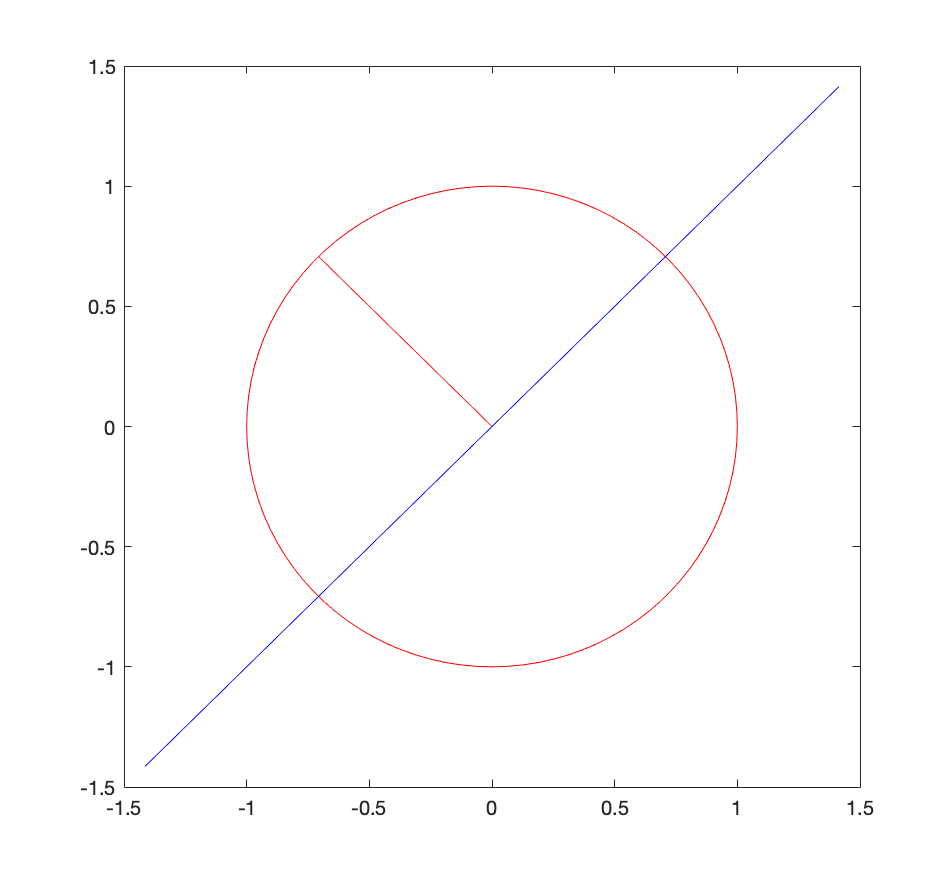
\includegraphics[width=.75\textwidth]{plot5.png}
            \end{center}
          \end{figure}
\end{exercise}











\end{document}




















